\documentclass[12pt, a4paper]{report}
\usepackage{graphicx}
\renewcommand*\contentsname{Table Of Contents}
\begin{document}
\begin{titlepage}
\begin{center}
\vfill
\Large{\textbf{KANTIPUR ENGINEERING COLLEGE}}\\
\large{\textbf{(Affiliated to Tribhuvan University)}}\\
\large{\textbf{Dhapakhel, Lalitpur}}\\
\vfill	%vertically fill the space 


\includegraphics[scale=1]{logo.png}

\vfill
\large{\textbf{[Subject Code:EX 755]}}\\ %Change This Line
\large{\textbf{A MAJOR PROJECT  REPORT ON  }}\\ %Change This Line
\Large{\textbf{PNEUMONIA DETECTION USING X-RAY  }}\\

\vfill	%vertically fill the space 
\large{\textbf{Submitted by:}}\\

{\normalsize Aashish Parajuli [90/bct/073]\\
Shashank Thapa  [126/bct/073]\\
Nischal Sagar Shrestha  [116/bct/073]\\ 
Kritika Baral [27/bct/073]\\
}


\vfill	%vertically fill the space 
\textbf{A MAJOR PROJECT SUBMITTED IN PARTIAL FULFILLMENT OF THE REQUIREMENT FOR THE DEGREE OF BACHELOR IN COMPUTER ENGINEERING}\\

\vfill	%vertically fill the space 
\large{\textbf{Submitted to:\\
Department of Computer and Electronics Engineering}}\\
\vfill
\today	
\vfill
\pagebreak
\newpage

\large{\textbf{PNEUMONIA DETECTION USING X-RAY}}\\
\vfill
\large{\textbf{Submitted by:}}\\
{\normalsize Aashish Parajuli [90/bct/073]\\
Shashank Thapa  [126/bct/073]\\
Nischal Sagar Shrestha [116/bct/073]\\ 
Kritika Baral [27/bct/073]\\
}
\vfill
\large{\textbf{Supervised by:}}\\
{\normalsize Aashish Parajuli [90/bct/073]\\
Shashank Thapa {14pt} [126/bct/073]\\

}
\vfill	%vertically fill the space 
\textbf{A MAJOR PROJECT SUBMITTED IN PARTIAL FULFILLMENT OF THE REQUIREMENT FOR THE DEGREE OF BACHELOR IN COMPUTER ENGINEERING}\\

\vfill	%vertically fill the space 
\large{\textbf{Submitted to:\\
Department of Computer and Electronics Engineering}}\\
\vfill

\end{center}
\end{titlepage}


\chapter*{Abstract}

We will be developing a web app that uses Convolutional Neural Network that is trained from scratch to detect and identify the probability of presence of pneumonia in a patient using their chest X-rays. The images of the X-rays will be taken from kaggle and will be given to the Neural Network as set of training images. The images will be subjected to basic transformations such as down scaling, skewing and rotations on the basis of the processing power at hand. Based on these images the CNN will identify whether the patient has pneumonia or not. We will be using python and django as the web framework to create the web app, in addition to this we will be using Keras and Tensorflow libraries to help us model the Neural Network and scikit-learn and matplotlib for the prediction models. This model could help mitigate the reliability and interpretability challenges often faced when dealing with medical imagery. We believe that the application of automated methods will help in early diagnosis.

Keywords - Image Processing, Convolutional Neural Network, Pneumonia, Automated Disease Diagnosis
\listoffigures
\tableofcontents
\newpage

\chapter{Introduction}
\section{Background}

Pneumonia is a life-threatening infectious disease affecting one or both lungs in humans. Bacterias, viruses and fungi are all the organisms that can cause Pneumonia. Streptococcus pneumoniae is the most common cause of bacterial Pneumonia whereas influenza is the leading cause of viral Pneumonia. Although the severity of Pneumonia can vary, young children, seniors and people with weakened immune system are the most vulnerable. The CDC reports that 1 million people are hospitalized due to Pneumonia every year and unfortunately, 50,000 people die due to Pneumonia every year. Early and proper diagnosis is key to decreasing the mortality rate of patients. Conventional diagnosis method like solely examining the patients medical history or symptoms have their shortcomings. Chest X-Rays have long been the most reliable method of diagnosis for Pneumonia. Although these tools are reliable, human error can always be a possibility which can be severe as the life of the patient is in the line.

pneumonia is an air-space disease, the cause of Pneumonia could be bacteria, viruses or fungi that could be present in the patient’s air-spaces which are naked to the human eye. A diagnosis of pneumonia is done by studying the presence of infiltrates, or white spots, the loss of diaphragmatic shadows or areas of the lungs that are filled with liquid instead of air in the X-Ray.

Chest X-Rays which are used to diagnose pneumonia need expert radiotherapists for evaluation. Thus, developing an automatic system for detecting pneumonia would be beneficial for treating the disease without any delay, particularly in remote areas. However, examining chest X-Rays is not a leisurely task for radiotherapists. In chest X-ray images, the appearance of pneumonia can be hazy and can be misapprehended with other diagnoses. The evaluation of chest X-Ray specifically in case of Pneumonia can be misleading because many other problems like congestive heart failure, lung scarring etc. can mimic a Pneumonia. This is the main reason behind the misclassification of the X-ray images in the dataset. Thus, the task is challenging and the development of an algorithm for detecting thoracic diseases like Pneumonia would increase the accessibility of clinical settings in remote areas as well. 

All the radio-images used in this project will be classified into three types; training images, test images and validation images. Depending on the processing power that is utilized for training the neural network, the images will be downscaled and transformed if necessary to a more suitable resolution. Since the output of the system will be a binary output that is either the patient has pneumonia or they don’t, we will be labelling the normal X-rays as ‘1’ and the X-rays of patients with pneumonia as ‘0’.

Due to the success of deep learning algorithms in analyzing medical images, Convolutional Neural Networks (CNNs) have gained much attention for disease classification. In addition, features learned by pre-trained CNN models on large-scale datasets are much useful in image classification tasks.

\section{Problem statement}

As remote areas do not have the privilege of radiotherapists being able to properly diagnose pneumonia in the early stage, it is one of the most prevalent communicable disease that is life threatening. Early diagnosis of Pneumonia can help cure it and secure the well being of the patient, but the lack of radiotherapists and the possibility of human error in detecting or misinterpreting the disease can cause the life of a patient. Hence it is a serious matter of urgency that the diagnosis is as accurate as possible.

\section{Objective}
\begin{enumerate}
\item   To identify pneumonia by studying chest X-Rays as accurately as possible
\item	To minimize human error in diagnosis and analysis of chest X-Rays
\end{enumerate}

\section{Application}
The main application area for this project will be in remote areas where radiotherapists will not be present at a moment’s notice. It is also applicable when there is uncertainty in the type of Pneumonia that is present in the patient. As pollution is increasing day by day and the air-space is being littered with more and more bacteria, viruses and other microorganisms the possibility of air-space diseases such as Pneumonia is increasing. Although the annual deaths caused by Pneumonia has decreased significantly over the period of time, it is still one of the main causes of deaths throughout the globe. Fortunately, with the growth of Neural Networks and advancement in image processing, it has been easier to use these technologies to aid the medical field with our projects.
\section{Project features}
\section{Feasibility Analysis}

\subsection{Economical Feasibility }

\subsection{Technical Feasibility}
As technology can be termed as a basic need of an individual in the current context people are quite familiar with it. So our application will be very simple as a simple UI will be implemented in our application, so it will be technically feasible to an individual. 

\subsection{Operational Feasibility}
An image of the X-Ray is enough to be tested by the system. No any vast components and methods will be implemented in the UI. A simple send button will be implemented so a basic user can operate this system easily. So it can be operationally feasible.
\section{System Requirement}
\subsection{Software Requirement}
Operating Systems: Ubuntu Linux , or Mac OS, or Windows 
 IDE for Python and Machine Learning Python Libraries.

\pagebreak
\chapter{Literature Review}

As Pneumonia is one of the most dangerous air-space diseases there are various methods to diagnose this successfully blood test, pulse oximetry test and sputum tests are a few examples. But these tests take time and are intrusive in comparison to chest X-Ray analysis which is the most reliable and the most efficient diagnostic method. As stated above, manual analysis of these X-Rays is not a leisurely task for the radiotherapists and has its own shortcomings. In order to eliminate or minimize these shortcomings automated diagnostic systems are being used.

\section{Existing System}
In recent time, exploration of Machine learning algorithms in detecting thoracic diseases has gained attention in research area of medical image classification. Lakhani and Sundaram (2017) proposed a method of detecting pulmonary tuberculosis following the architecture of two different DCNNs AlexNet and GoogleNet. Lung nodule classification mainly for diagnosing lung cancer proposed by Huang et al. also adopted deep learning techniques. Performance of different variants of Convolutional Neural Networks (CNNs) for abnormality detection in chest X-Rays was proposed by Islam et al. using the publicly available OpenI dataset. For the better exploration of machine learning in chest screening, Wang et al. (2017) released a larger dataset of frontal chest X-Rays. Recently, Pranav Rajpurkar, Jeremy Irvin, et al. (2017) explored this dataset for detecting pneumonia at a level better than radiologists, they referred their model as ChexNet which uses DenseNet-121 layer architecture for detecting all the 14 diseases from a lot of 112,200 images available in the dataset. After the CheXNet model, Benjamin Antin et al.(2017) worked on the same dataset and proposed a logistic regression model for detecting pneumonia. Pulkit Kumar, Monika Grewal (2017) using the cascading convolutional networks contributed their research for multilabel classification of thoracic diseases. Zhe Li (2018) recently proposed a convolutional network model for disease identification and localization.
Latest improvements in deep learning models and the availability of huge datasets have assisted algorithms to outperform medical personnel in numerous medical imaging tasks such as skin cancer classification, hemorrhage identification, arrhythmia detection, and diabetic retinopathy detection. Automated diagnoses enabled by chest radiographs have received growing interests. .ese algorithms are increasingly being used for conducting lung nodule detection and pulmonary tuberculosis classification. The performance of several convolutional models on diverse abnormalities relying on the publicly available OpenI dataset found that the same deep convolutional network architecture does not perform well across all abnormalities, ensemble models significantly improved classification accuracy when compared with single model, and finally, deep learning method improved accuracy when compared to rule-based methods. Statistical dependency between labels was studied to arrive at more precise predictions, thereby outperforming other techniques on given 13 images selected from 14 classes. Algorithms for mining and predicting labels emanating from radiology images as well as reports have been studied, but the image labels were generally constrained to disease tags, thus lacking contextual information. Detection of diseases from X-ray images was examined in, classifications on image views from chest X-ray were carried out, and body parts segmentation from chest X-ray images and computed tomography was performed in. Conversely, learning image features from text and creating image descriptions relative to what a human would describe are yet to be exploited.

\vfill
\pagebreak
\chapter{Methodology}
The architecture of the proposed model will be divided into three different stages - the preprocessing stage, the feature extraction stage and the classification stage. 
\begin{enumerate}

\item
The Pre-Processing Stage:\\
The primary goal of using Convolutional Neural Network in most of the image classification tasks is to reduce the computational complexity of the model which is likely to increase if the input are images . The original 3-channel images will be resized to 224×224 pixels to reduce the heavy computation and for faster processing. All of the further techniques will be applied over these downsized images. 

\item
Feature extraction stage:\\
Each layer in the feature extraction layer will take its immediate preceding layer's output as input, and its output will be passed as an input to the succeeding layers. The rescale operation represents image reduction or magnification during the augmentation process. The rotation range denotes the range in which the images will be randomly rotated during training, i.e., 40 degrees. Width shift is the horizontal translation of the images by 0.2 percent, and height shift is the vertical translation of the images by 0.2 percent. In addition, a shear range of 0.2 percent clips the image angles in a counterclockwise direction. The zoom range randomly zooms the images to the ratio of 0.2 percent, and finally, the images will be flipped horizontally.

\item
Classification stage:\\
The classifier will be placed at the far end of the proposed convolutional neural network (CNN) model. It is simply an artificial neural network (ANN) often referred to as a dense layer. This classifier will require individual features (vectors) to perform computations like any other classifier. Therefore, the output of the feature extractor (CNN part) will be converted into a 1D feature vector for the classifiers. This process is called flattening where the 2D plane from the CNN feature extraction will be flattened into a 1D plane. The classification layer will contain a flattened layer, a dropout of size 0.5, two dense layers of size 512 and 1, respectively, a Rectified Linear Unit between the two dense layers and a sigmoid activation function that performs the classification tasks.


\end{enumerate}
\vfill
\begin{figure}
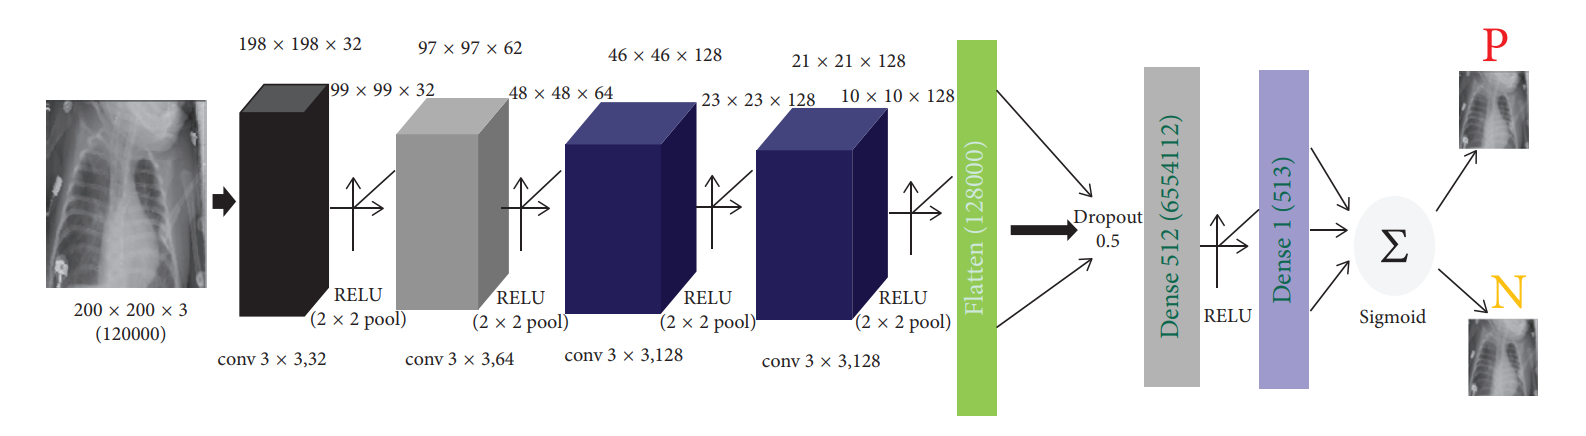
\includegraphics[width=350 pt ,height=150 pt]{pic.png}
\caption{Figure of Proposed system \label{fig:3.1}}
\end{figure}
\section{Software Development Model}
\subsection{Spiral Development Model}
The spiral model is a risk-driven software development process model.Based on the
unique risk patterns of a given project,the spiral model guides a team to adopt elements
of one or more process models , such as incremental, waterfall,or evolutionary prototyping.

\begin{figure}
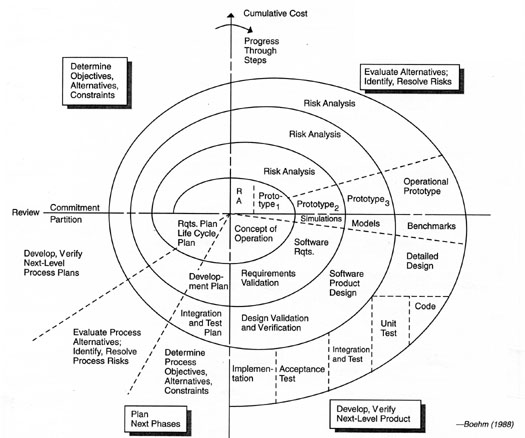
\includegraphics[scale = 3]{spiral.jpg}
\caption{Figure of Spiral Development Model.\label{fig:3.2}}
\end{figure}
\vfill
\pagebreak
\section{System Flow Chart}
\begin{figure}
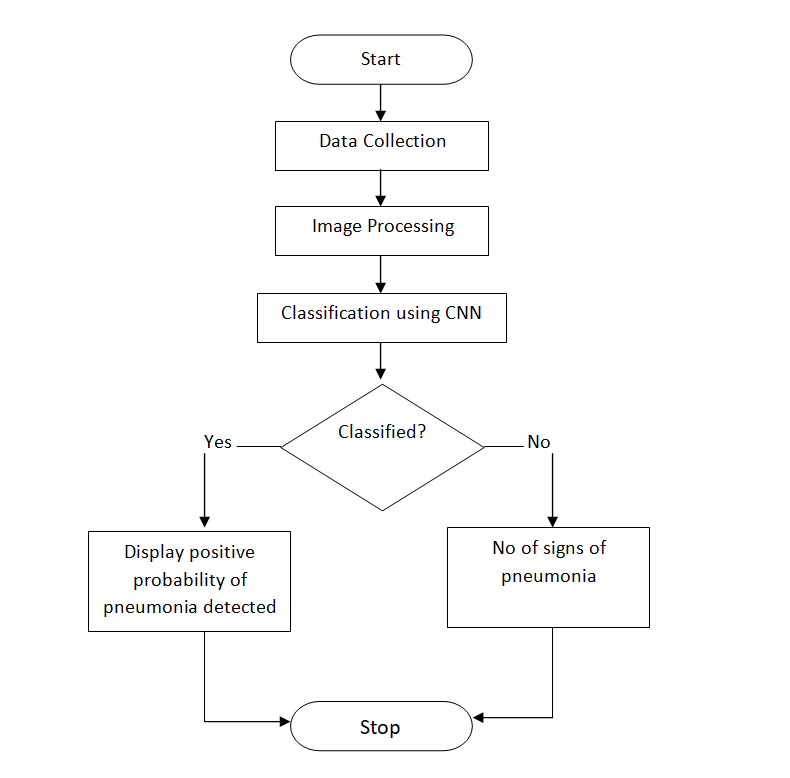
\includegraphics[width=350 pt ,height=500 pt]{system.png}\caption{Figure of System Flow Chart \label{fig:3.3}}
\end{figure}
\vfill


\chapter{Work Schedule}



\chapter*{References}



\end{document}
